% Source: AESP_466_ClassWork/Assignments/Assignment_3/textbook_example_problems/E6.2/fuselage_tikz.tex
\documentclass[tikz,border=10pt]{standalone}
\usepackage{tikz}
\usetikzlibrary{arrows.meta}

\begin{document}
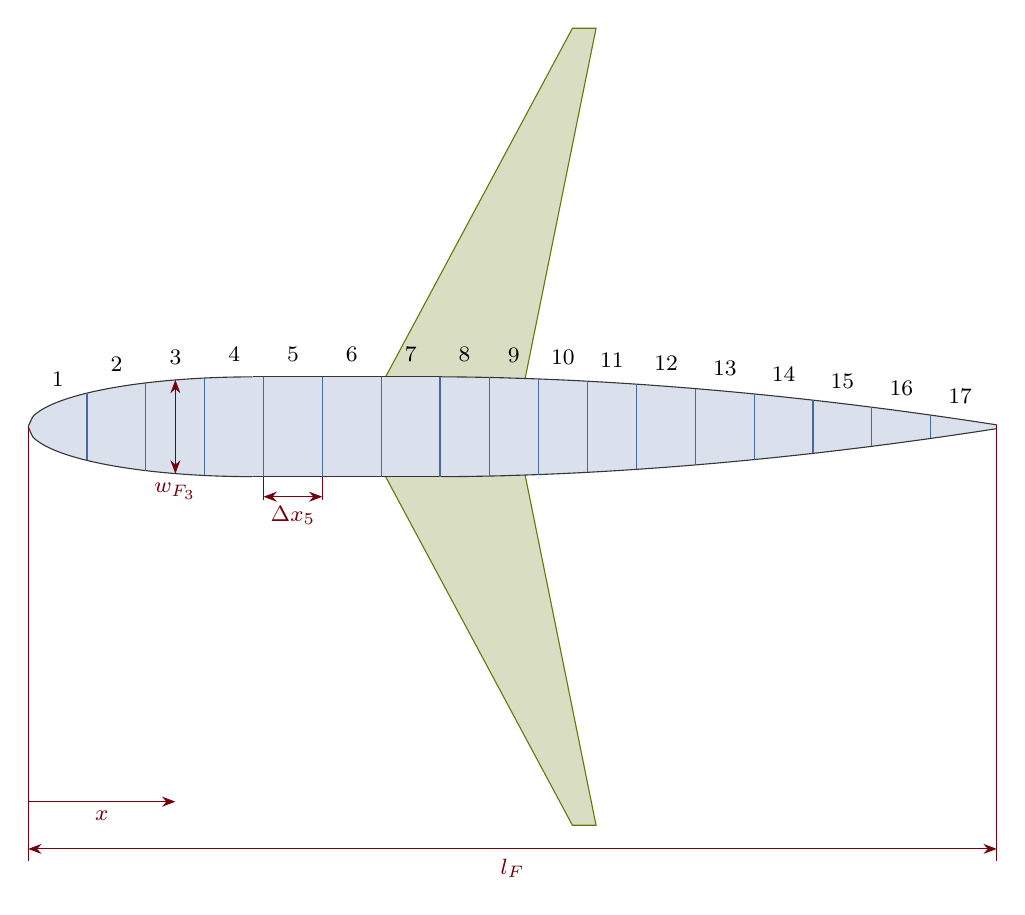
\begin{tikzpicture}[>=Stealth, xscale=0.3, yscale=0.15]

% Define colors using brand palette
\definecolor{garnet}{RGB}{115,0,10}
\definecolor{black90}{RGB}{54,54,54}
\definecolor{atlantic}{RGB}{70,106,159}
\definecolor{horseshoe}{RGB}{101,120,11}

% ============================================
% FUSELAGE GEOMETRY PARAMETERS
% ============================================
\def\Lnose{9.5}        % nose cone length
\def\Lconst{8}         % constant section length
\def\Ltail{23.5}       % tail cone length
\def\Ltotal{41}        % total fuselage length
\def\Rmax{2.64}        % max half-width
\def\Rtail{0.1}        % tail end half-width
\def\ws{1.6}           % width scale factor
\pgfmathsetmacro{\xtailstart}{\Lnose + \Lconst}

% ============================================
% WINGS (drawn first, behind fuselage)
% ============================================
\def\wingroot{15}        % x position of wing root (section 7 area)
\def\wingrootchord{6}    % root chord length
\def\wingsemispan{30}    % half wingspan
\def\wingsweep{15}       % leading edge sweep angle (degrees)
\def\wingtipchord{1}     % tip chord length

\pgfmathsetmacro{\wingattachy}{\Rmax - 0.3}
\pgfmathsetmacro{\wingtipoffset}{\wingsemispan * tan(\wingsweep)}

% Right wing
\fill[horseshoe!25]
    (\wingroot, {\ws*\wingattachy}) --
    (\wingroot + \wingtipoffset, {\ws*\wingattachy + \wingsemispan}) --
    (\wingroot + \wingtipoffset + \wingtipchord, {\ws*\wingattachy + \wingsemispan}) --
    (\wingroot + \wingrootchord, {\ws*\wingattachy}) -- cycle;
\draw[horseshoe]
    (\wingroot, {\ws*\wingattachy}) --
    (\wingroot + \wingtipoffset, {\ws*\wingattachy + \wingsemispan}) --
    (\wingroot + \wingtipoffset + \wingtipchord, {\ws*\wingattachy + \wingsemispan}) --
    (\wingroot + \wingrootchord, {\ws*\wingattachy}) -- cycle;

% Left wing
\fill[horseshoe!25]
    (\wingroot, {-\ws*\wingattachy}) --
    (\wingroot + \wingtipoffset, {-\ws*\wingattachy - \wingsemispan}) --
    (\wingroot + \wingtipoffset + \wingtipchord, {-\ws*\wingattachy - \wingsemispan}) --
    (\wingroot + \wingrootchord, {-\ws*\wingattachy}) -- cycle;
\draw[horseshoe]
    (\wingroot, {-\ws*\wingattachy}) --
    (\wingroot + \wingtipoffset, {-\ws*\wingattachy - \wingsemispan}) --
    (\wingroot + \wingtipoffset + \wingtipchord, {-\ws*\wingattachy - \wingsemispan}) --
    (\wingroot + \wingrootchord, {-\ws*\wingattachy}) -- cycle;


% ============================================
% FUSELAGE FILL (light blue) - using saved path for clean fill
% ============================================
\path[save path=\fuselagepath]
    (0,0)
    % Nose (top) - elliptical profile
    \foreach \i in {1,...,50} {
        -- ({\Lnose*(1 - cos(\i*90/50))}, {\ws*\Rmax*sin(\i*90/50)})
    }
    % Constant section (top)
    -- ({\Lnose + \Lconst}, {\ws*\Rmax})
    % Tail (top) - power-law taper
    \foreach \i in {1,...,80} {
        -- ({\xtailstart + \i*\Ltail/80}, {\ws*(\Rmax - (\Rmax - \Rtail)*((\i/80)^1.8))})
    }
    % Tail cap
    -- (\Ltotal, {-\ws*\Rtail})
    % Tail (bottom) - power-law taper reversed
    \foreach \i in {80,79,...,1} {
        -- ({\xtailstart + \i*\Ltail/80}, {-\ws*(\Rmax - (\Rmax - \Rtail)*((\i/80)^1.8))})
    }
    % Constant section (bottom)
    -- (\Lnose, {-\ws*\Rmax})
    % Nose (bottom) - elliptical profile reversed
    \foreach \i in {50,49,...,1} {
        -- ({\Lnose*(1 - cos(\i*90/50))}, {-\ws*\Rmax*sin(\i*90/50)})
    }
    -- cycle;

\fill[atlantic!20, use path=\fuselagepath];

% ============================================
% FUSELAGE OUTLINE
% ============================================
% Nose
\draw[black90, domain=0:\Lnose, samples=50, smooth]
    plot (\x, {\ws * \Rmax * sqrt(1 - ((\Lnose - \x)/\Lnose)^2)});
\draw[black90, domain=0:\Lnose, samples=50, smooth]
    plot (\x, {-\ws * \Rmax * sqrt(1 - ((\Lnose - \x)/\Lnose)^2)});

% Constant section
\draw[black90] (\Lnose, {\ws*\Rmax}) -- ({\Lnose + \Lconst}, {\ws*\Rmax});
\draw[black90] (\Lnose, {-\ws*\Rmax}) -- ({\Lnose + \Lconst}, {-\ws*\Rmax});

% Tail
\draw[black90, domain=\xtailstart:\Ltotal, samples=80, smooth]
    plot (\x, {\ws * (\Rmax - (\Rmax - \Rtail) * ((\x - \xtailstart)/\Ltail)^1.8)});
\draw[black90, domain=\xtailstart:\Ltotal, samples=80, smooth]
    plot (\x, {-\ws * (\Rmax - (\Rmax - \Rtail) * ((\x - \xtailstart)/\Ltail)^1.8)});

% Tail cap
\draw[black90] (\Ltotal, {\ws*\Rtail}) -- (\Ltotal, {-\ws*\Rtail});

% ============================================
% SECTION DIVIDING LINES (blue)
% ============================================
% Nose section boundaries
\pgfmathsetmacro{\yOne}{  \Rmax * sqrt(1 - ((\Lnose - 2.49)/\Lnose)^2)}
\pgfmathsetmacro{\yTwo}{  \Rmax * sqrt(1 - ((\Lnose - 4.98)/\Lnose)^2)}
\pgfmathsetmacro{\yThree}{\Rmax * sqrt(1 - ((\Lnose - 7.47)/\Lnose)^2)}

\draw[atlantic] (2.49, {\ws*\yOne}) -- (2.49, {-\ws*\yOne});
\draw[atlantic] (4.98, {\ws*\yTwo}) -- (4.98, {-\ws*\yTwo});
\draw[atlantic] (7.47, {\ws*\yThree}) -- (7.47, {-\ws*\yThree});

% Constant section boundaries
\draw[atlantic] (9.96, {\ws*\Rmax}) -- (9.96, {-\ws*\Rmax});
\draw[atlantic] (12.45, {\ws*\Rmax}) -- (12.45, {-\ws*\Rmax});
\draw[atlantic] (14.94, {\ws*\Rmax}) -- (14.94, {-\ws*\Rmax});
\draw[atlantic] (17.43, {\ws*\Rmax}) -- (17.43, {-\ws*\Rmax});

% Tail section boundaries
\pgfmathsetmacro{\yEight}{   \Rmax - (\Rmax - \Rtail) * ((19.51 - \xtailstart)/\Ltail)^1.8}
\pgfmathsetmacro{\yNine}{    \Rmax - (\Rmax - \Rtail) * ((21.59 - \xtailstart)/\Ltail)^1.8}
\pgfmathsetmacro{\yTen}{     \Rmax - (\Rmax - \Rtail) * ((23.67 - \xtailstart)/\Ltail)^1.8}
\pgfmathsetmacro{\yEleven}{  \Rmax - (\Rmax - \Rtail) * ((25.75 - \xtailstart)/\Ltail)^1.8}
\pgfmathsetmacro{\yTwelve}{  \Rmax - (\Rmax - \Rtail) * ((28.24 - \xtailstart)/\Ltail)^1.8}
\pgfmathsetmacro{\yThirteen}{\Rmax - (\Rmax - \Rtail) * ((30.73 - \xtailstart)/\Ltail)^1.8}
\pgfmathsetmacro{\yFourteen}{\Rmax - (\Rmax - \Rtail) * ((33.22 - \xtailstart)/\Ltail)^1.8}
\pgfmathsetmacro{\yFifteen}{ \Rmax - (\Rmax - \Rtail) * ((35.71 - \xtailstart)/\Ltail)^1.8}
\pgfmathsetmacro{\ySixteen}{ \Rmax - (\Rmax - \Rtail) * ((38.20 - \xtailstart)/\Ltail)^1.8}

\draw[atlantic] (19.51, {\ws*\yEight}) -- (19.51, {-\ws*\yEight});
\draw[atlantic] (21.59, {\ws*\yNine}) -- (21.59, {-\ws*\yNine});
\draw[atlantic] (23.67, {\ws*\yTen}) -- (23.67, {-\ws*\yTen});
\draw[atlantic] (25.75, {\ws*\yEleven}) -- (25.75, {-\ws*\yEleven});
\draw[atlantic] (28.24, {\ws*\yTwelve}) -- (28.24, {-\ws*\yTwelve});
\draw[atlantic] (30.73, {\ws*\yThirteen}) -- (30.73, {-\ws*\yThirteen});
\draw[atlantic] (33.22, {\ws*\yFourteen}) -- (33.22, {-\ws*\yFourteen});
\draw[atlantic] (35.71, {\ws*\yFifteen}) -- (35.71, {-\ws*\yFifteen});
\draw[atlantic] (38.20, {\ws*\ySixteen}) -- (38.20, {-\ws*\ySixteen});

% ============================================
% SECTION NUMBERS
% ============================================
\def\labeloffset{0.3}

\pgfmathsetmacro{\ySone}{\Rmax * sqrt(1 - ((\Lnose - 1.25)/\Lnose)^2)}
\node[above, font=\footnotesize] at (1.25, {\ws*(\ySone + \labeloffset)}) {1};

\pgfmathsetmacro{\yStwo}{\Rmax * sqrt(1 - ((\Lnose - 3.74)/\Lnose)^2)}
\node[above, font=\footnotesize] at (3.74, {\ws*(\yStwo + \labeloffset)}) {2};

\pgfmathsetmacro{\ySthree}{\Rmax * sqrt(1 - ((\Lnose - 6.23)/\Lnose)^2)}
\node[above, font=\footnotesize] at (6.23, {\ws*(\ySthree + \labeloffset)}) {3};

\pgfmathsetmacro{\ySfour}{\Rmax * sqrt(1 - ((\Lnose - 8.72)/\Lnose)^2)}
\node[above, font=\footnotesize] at (8.72, {\ws*(\ySfour + \labeloffset)}) {4};

\node[above, font=\footnotesize] at (11.21, {\ws*(\Rmax + \labeloffset)}) {5};
\node[above, font=\footnotesize] at (13.70, {\ws*(\Rmax + \labeloffset)}) {6};
\node[above, font=\footnotesize] at (16.19, {\ws*(\Rmax + \labeloffset)}) {7};

\pgfmathsetmacro{\ySeight}{\Rmax - (\Rmax - \Rtail) * ((18.47 - \xtailstart)/\Ltail)^1.8}
\node[above, font=\footnotesize] at (18.47, {\ws*(\ySeight + \labeloffset)}) {8};

\pgfmathsetmacro{\ySnine}{\Rmax - (\Rmax - \Rtail) * ((20.55 - \xtailstart)/\Ltail)^1.8}
\node[above, font=\footnotesize] at (20.55, {\ws*(\ySnine + \labeloffset)}) {9};

\pgfmathsetmacro{\ySten}{\Rmax - (\Rmax - \Rtail) * ((22.63 - \xtailstart)/\Ltail)^1.8}
\node[above, font=\footnotesize] at (22.63, {\ws*(\ySten + \labeloffset)}) {10};

\pgfmathsetmacro{\ySeleven}{\Rmax - (\Rmax - \Rtail) * ((24.71 - \xtailstart)/\Ltail)^1.8}
\node[above, font=\footnotesize] at (24.71, {\ws*(\ySeleven + \labeloffset)}) {11};

\pgfmathsetmacro{\yStwelve}{\Rmax - (\Rmax - \Rtail) * ((27.00 - \xtailstart)/\Ltail)^1.8}
\node[above, font=\footnotesize] at (27.00, {\ws*(\yStwelve + \labeloffset)}) {12};

\pgfmathsetmacro{\ySthirteen}{\Rmax - (\Rmax - \Rtail) * ((29.49 - \xtailstart)/\Ltail)^1.8}
\node[above, font=\footnotesize] at (29.49, {\ws*(\ySthirteen + \labeloffset)}) {13};

\pgfmathsetmacro{\ySfourteen}{\Rmax - (\Rmax - \Rtail) * ((31.98 - \xtailstart)/\Ltail)^1.8}
\node[above, font=\footnotesize] at (31.98, {\ws*(\ySfourteen + \labeloffset)}) {14};

\pgfmathsetmacro{\ySfifteen}{\Rmax - (\Rmax - \Rtail) * ((34.47 - \xtailstart)/\Ltail)^1.8}
\node[above, font=\footnotesize] at (34.47, {\ws*(\ySfifteen + \labeloffset)}) {15};

\pgfmathsetmacro{\ySsixteen}{\Rmax - (\Rmax - \Rtail) * ((36.96 - \xtailstart)/\Ltail)^1.8}
\node[above, font=\footnotesize] at (36.96, {\ws*(\ySsixteen + \labeloffset)}) {16};

\pgfmathsetmacro{\ySseventeen}{\Rmax - (\Rmax - \Rtail) * ((39.45 - \xtailstart)/\Ltail)^1.8}
\node[above, font=\footnotesize] at (39.45, {\ws*(\ySseventeen + \labeloffset)}) {17};

% ============================================
% VERTICAL REFERENCE LINES AT NOSE AND TAIL
% ============================================
\draw[garnet] (0, 0) -- (0, {-\ws*(\wingattachy + \wingsemispan) + 15});
\draw[garnet] (\Ltotal, {\ws*\Rtail}) -- (\Ltotal, {-\ws*(\wingattachy + \wingsemispan) + 15});

% Total fuselage length dimension
\draw[<->, garnet] (0, {-\ws*(\wingattachy + \wingsemispan) + 16}) -- (\Ltotal, {-\ws*(\wingattachy + \wingsemispan) + 16})
    node[midway, below, font=\footnotesize] {$l_F$};

% X-direction indicator arrow
\draw[->, garnet] (0, {-\ws*(\wingattachy + \wingsemispan) + 20}) -- (6.23, {-\ws*(\wingattachy + \wingsemispan) + 20})
    node[midway, below, font=\footnotesize] {$x$};

% ============================================
% INTERNAL WIDTH DIMENSION FOR SECTION 3
% ============================================
\pgfmathsetmacro{\yWthree}{\Rmax * sqrt(1 - ((\Lnose - 6.23)/\Lnose)^2)}
\draw[<->, garnet] (6.23, {\ws*\yWthree}) -- (6.23, {-\ws*\yWthree})
    node[below, font=\footnotesize] {$w_{F_3}$};

% ============================================
% DIMENSION FOR SECTION 5
% ============================================
\def\dimoffset{2.0}
% Extension lines
\draw[garnet] (9.96, {-\ws*\Rmax}) -- (9.96, {-\ws*\Rmax - \dimoffset});
\draw[garnet] (12.45, {-\ws*\Rmax}) -- (12.45, {-\ws*\Rmax - \dimoffset});
% Dimension line with arrows
\draw[<->, garnet] (9.96, {-\ws*\Rmax - \dimoffset + 0.3}) -- (12.45, {-\ws*\Rmax - \dimoffset + 0.3})
    node[midway, below, font=\footnotesize] {$\Delta x_5$};

\end{tikzpicture}
\end{document}
